% Floor on the line: 2.3 falls in [2,3), and -1.2 falls in [-2,-1).
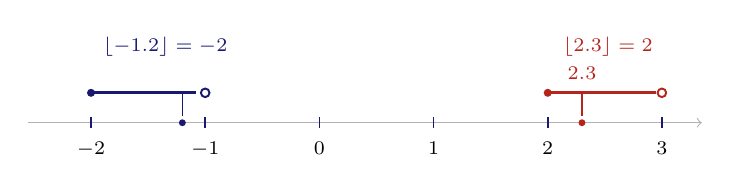
\begin{tikzpicture}[x=1.45cm,y=1cm]
  \draw[gray!60,->] (-2.55,0) -- (3.35,0);
  \foreach \n in {-2,-1,0,1,2,3} {
    \draw[MidnightBlue,line width=0.6pt] (\n,0.07) -- (\n,-0.07);
    \node[font=\scriptsize,anchor=north] at (\n,-0.12) {$\n$};
  }
  % [2, 3): 2.3
  \draw[BrickRed,line width=1.05pt] (2,0.38) -- (2.95,0.38);
  \fill[BrickRed] (2,0.38) circle (1.45pt);
  \draw[BrickRed,line width=0.7pt] (3,0.38) circle (1.55pt);
  \fill[BrickRed] (2.3,0) circle (1.25pt);
  \draw[BrickRed,thin] (2.3,0.08) -- (2.3,0.38);
  \node[font=\scriptsize,BrickRed,anchor=south] at (2.3,0.42) {$2.3$};
  \node[font=\scriptsize,BrickRed,anchor=south west] at (2.05,0.72) {$\lfloor 2.3\rfloor=2$};
  % [-2, -1): -1.2
  \draw[MidnightBlue,line width=1.05pt] (-2,0.38) -- (-1.08,0.38);
  \fill[MidnightBlue] (-2,0.38) circle (1.45pt);
  \draw[MidnightBlue,line width=0.7pt] (-1,0.38) circle (1.55pt);
  \fill[MidnightBlue] (-1.2,0) circle (1.25pt);
  \draw[MidnightBlue,thin] (-1.2,0.08) -- (-1.2,0.38);
  \node[font=\scriptsize,MidnightBlue,anchor=south] at (-1.35,0.72) {$\lfloor -1.2\rfloor=-2$};
\end{tikzpicture}
